
\begin{frame}[t]{Modelos de simulación de la ecología del vector.}
  \begin{center}
   \begin{columns}[T]
        \begin{column}[T]{4cm}
             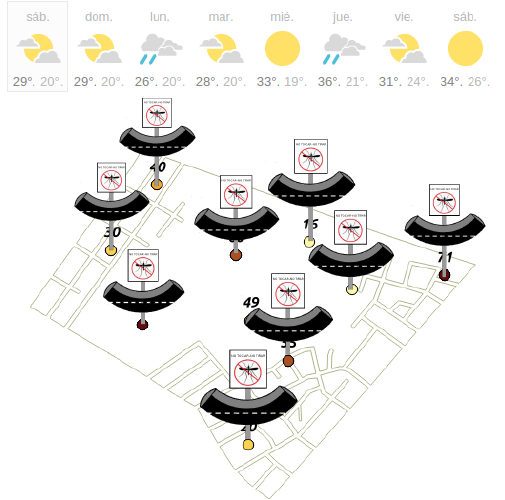
\includegraphics[width=4.5cm]{./graphics/larvitrmpas-clima.png}
        \end{column}
        \begin{column}[T]{7cm}
          \begin{itemize}
          \item Larvitrampas como puntos de control.
          \item Combinar información regionalizada, meteorológica y geográfica.
          \item Influencia de las variaciones climáticas.
          \item Simular el comportamiento del vector.
          \item Detección temprana de posibles focos y en consecuencia una posible epidemia.
          \item Conteo de larvas mediante PDI.
          \end{itemize}
        \end{column}
    \end{columns}
  \end{center}
\end{frame}

\begin{frame}[t]{Modelos de simulación de la ecología del vector.\\\textit{Modelo matemático del ciclo de vida.}}
  \begin{center}
   \begin{columns}[t]
        \begin{column}[T]{7cm}
            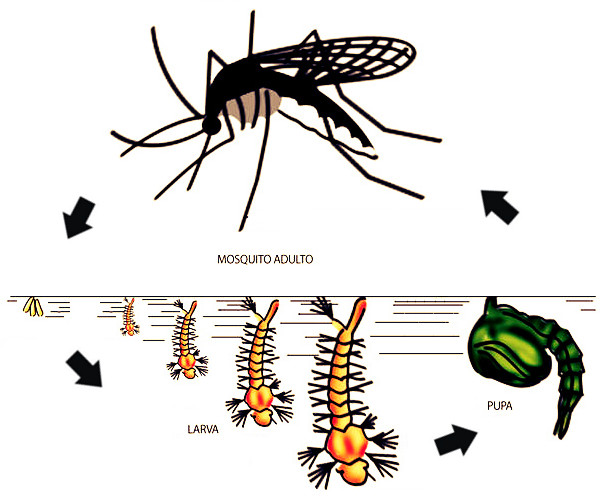
\includegraphics[width=7cm]{./graphics/ciclo-de-vida.jpg}
        \end{column}
        \begin{column}[T]{4cm}
          \begin{itemize}
            \item Tasas de desarrollo.
            \item Tasas de mortalidad.
            \item Dispersión.
            \item Ciclo gonotrófico.
            \item Ovipostura.
          \end{itemize}
        \end{column}
    \end{columns}
  \end{center}
\end{frame}

\begin{frame}[c]{Modelos de simulación de la ecología del vector.\\\textit{Modelo matemático del ciclo de vida.}}
  \begin{center}
   \begin{columns}[T]
        \begin{column}[T]{6cm}
            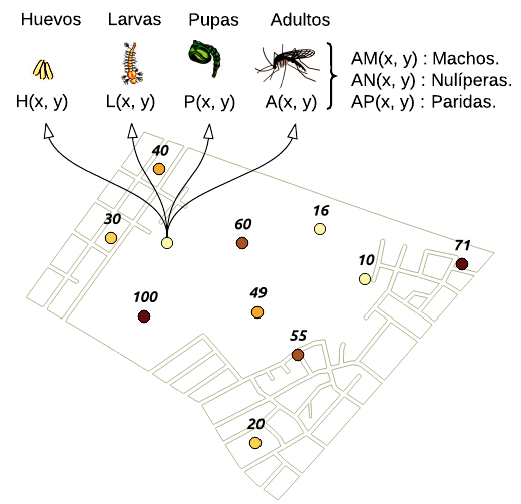
\includegraphics[width=6cm]{./graphics/modelado-poblacion.png}
        \end{column}
        \begin{column}[T]{5.5cm}
          \begin{itemize}
            \item $H(x, y)$ : Huevos.
            \item $L(x, y)$ : Larvas.
            \item $P(x, y)$ : Pupas.
            \item $AM(x, y)$ : Adultos machos.
            \item $AN(x, y)$ : Hembras nulíperas.
            \item $AP(x, y)$ : Hembras paridas.
          \end{itemize}
        \end{column}
    \end{columns}
  \end{center}
\end{frame}


\begin{frame}[c]{Modelos de simulación de la ecología del vector.\\\textit{Zonificación.}}

  \begin{center}
   \begin{columns}[T]
        \begin{column}[T]{4cm}
              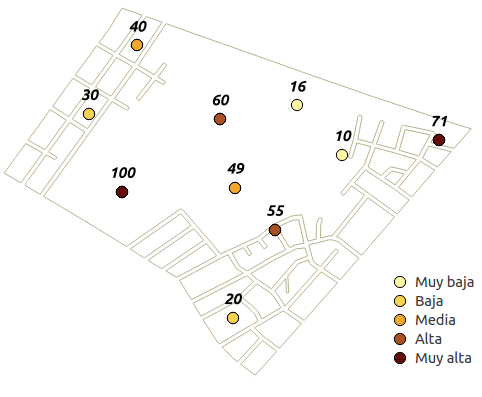
\includegraphics[width=\textwidth]{../book/capitulo-5/graphics/cartografia-vector.png}
        \end{column}
        \begin{column}[T]{6cm}
          \textit{\\Cada entorno puede contar con factores que lo hagan más o menos apto para el desarrollo, mortalidad, alimentación, dispersión y reproducción de individuos.}
        \end{column}
    \end{columns}
  \end{center}
\end{frame}

\begin{frame}[c]{Modelos de simulación de la ecología del vector.\\\textit{Zonificación.}}
  \begin{center}
   \begin{columns}[T]
        \begin{column}[T]{5cm}
            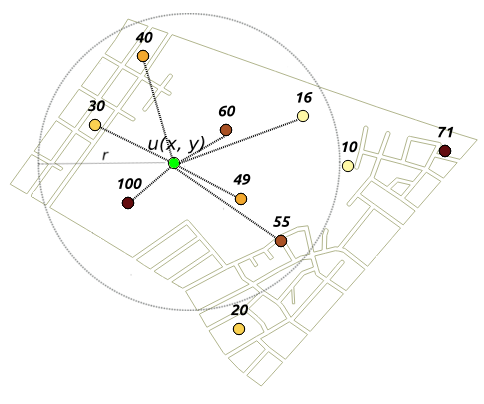
\includegraphics[width=5.5cm]{./graphics/zonificacion.png}
        \end{column}
        \begin{column}[T]{6cm}
          \begin{itemize}
          \item Los puntos de control permiten caracterizar la zona como más o menos apta para el desarrollo, mortalidad, alimentación, dispersión y reproducción.
          \item La población inicial se encuentra compuesta por larvas.
          \item Interpolación espacial para determinar la cantidad de larvas en $(x, y)$.
          \end{itemize}
        \end{column}
    \end{columns}
  \end{center}
\end{frame}


\begin{frame}[c]{Modelos de simulación de la ecología del vector.\\\textit{Zonificación.}}
  \begin{center}
   \begin{columns}[T]
        \begin{column}[T]{5cm}
			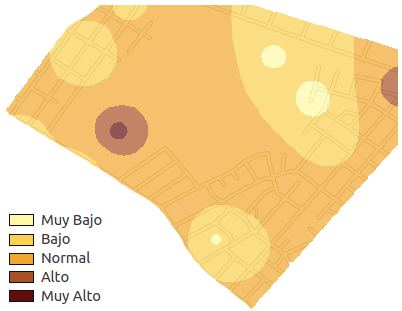
\includegraphics[width=\textwidth]{./graphics/zonificacion-intro.png}
        \end{column}
        \begin{column}[T]{6cm}
          \begin{itemize}
          \item Definir una escala de clasificación de las zonas.
          \item Establecer una relación entre la cantidad de larvas y el tipo de zona.
          \item Determinar el riesgo asociado a la cantidad de larvas.
          \item Estimar la cantidad de hembras con capacidad reproductiva, a partir de la cantidad de larvas.
          \end{itemize}
        \end{column}
    \end{columns}
  \end{center}
\end{frame}

\begin{frame}[c]{Modelos de simulación de la ecología del vector.\\\textit{Zonificación.}}
  Consideraciones para la clasificación de las zonas:
  \begin{itemize}
      \item El $50$ \% de las larvas observadas son hembras.
      \item La temperatura media anual es de 25 \textcelsius.
      \item La tasa mortalidad diaria natural de las larvas y pupas bajo optimas condiciones, a 25 \textcelsius, es igual a $0,01056\ \text{días}^{-1}$ respectivamente.
      \item El desarrollo, a 25 \textcelsius, de la larva hasta su emergencia a adulto es de $11,57$ días.
      \item El $32,10$ \% de las hembras adultas no oviponen.
  \end{itemize}
\end{frame}

\begin{frame}[t]{Modelos de simulación de la ecología del vector.\\\textit{Zonificación.}}

  \begin{table}
        \begin{minipage}{\textwidth}
          \centering
          \scriptsize
            \caption{\label{tab:cap4-puntaje-zona} Escala de clasificación de las zonas
            para el desarrollo, alimentación, dispersión y reproducción.}
            \begin{tabular}{l l c c c}
                \hline
                             & Niveles de & Mínimo$^a$ & Máximo$^a$  & Hembras$^b$ \\
                Tipo de zona & infestación & $u(x,y)$   & $u(x,y)$   & Reproductivas \\
                \hline
                \hline
                Pésima  & Muy bajo & 0  & 19 & 5 \\
                Mala    & Bajo     &20  & 35 & 10\\
                Regular & Medio    &36  & 51 & 15\\
                Buena   & Alto     &52  & 69 & 20\\
                Óptima  & Muy alto &70  & --$^c$ & --$^c$
            \end{tabular}
            \footnotetext[1]{\scriptsize Rango mínimo y máximo de $u(x,y)$ permitido para el tipo de zona.}
            \footnotetext[2]{\scriptsize Cantidad de hembras adultas con capacidad de oviponer.}
            \footnotetext[3]{\scriptsize No se estableció un límite superior para las zonas óptimas. }
        \end{minipage}
    \end{table}
\end{frame}

%Tasas de desarrollo.
\begin{frame}[c]{Modelos de simulación de la ecología del vector.\\\textit{Tasas de desarrollo.}}
  \begin{center}
   \begin{columns}[T]
        \begin{column}[T]{6.5cm}
            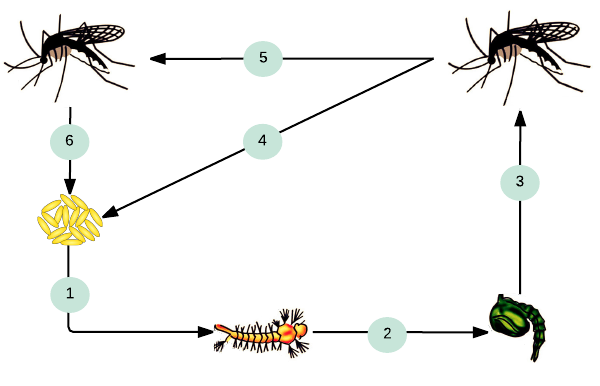
\includegraphics[width=7cm]{./graphics/tasas-desarrollo.png}
        \end{column}
        \begin{column}[T]{5cm}
          \begin{enumerate}
            \item Eclosión de huevos.
            \item Emergencia de pupas.
            \item Emergencia de adultos.
            \item Ciclo gonotrófico para hembras nulíperas.
            \item Ciclo gonotrófico para hembras paridas.
          \end{enumerate}
        \end{column}
    \end{columns}
  \end{center}
\end{frame}

\begin{frame}[t]{Modelos de simulación de la ecología del vector.\\\textit{Tasas de desarrollo
 (Sharpe y DeMichele, 1977).}}
  \begin{center}
      \begin{equation} \label{eq:schoolfield}
         R(k)  = R(298K) *\cfrac{ \cfrac{k}{298K} *
          exp \Bigg[
                  \cfrac{\Delta H_{A}}{R} \bigg(\cfrac{1}{298K} - \cfrac{1}{k}\bigg)
              \Bigg]}
          {1 + exp\Bigg[\cfrac{\Delta H_{H}}{R} \bigg(\cfrac{1}{T_{1/2}}- \cfrac{1}{k}\bigg)\Bigg] }
      \end{equation}
  \end{center}
   \begin{itemize}
      \item $R(k)$ : Tasa de desarrollo media ($dias^{-1}$).
      \item $\Delta H_{A}$ y $\Delta H_{H}$ : son entalpías termodinámicas características del organismo.
      \item $T_{1/2}$ es la temperatura cuando la mitad de la enzima se desactiva.
      \item $R$ : es la constante universal de los gases.
      \item $k$ : Temperatura en Kelvin.
    \end{itemize}
\end{frame}


\begin{frame}[c]{Modelos de simulación de la ecología del vector.\\\textit{Tasas de Mortalidad.}}
  \begin{itemize}
      \item Determinar la cantidad de individuos que deben ser eliminados de la población.
      \item Simular la reducción de la población por la mortalidad.
      \item La mortalidad depende de la etapa del ciclo de desarrollo:
      \begin{itemize}
		  \item Mortalidad de huevos $H(x, y)$.
		  \item Mortalidad de larvas $L(x,y)$.
		  \item Mortalidad de pupas $P(x,y)$.
		  \item Mortalidad de adultos $A(x,y)$.
      \end{itemize}
      \item La cantidad de individuos a eliminar debe ser entera.
  \end{itemize}
\end{frame}

\begin{frame}[c]{Modelos de simulación de la ecología del vector.\\\textit{Tasas de Mortalidad. (Otero et al., 2006)}}

  \begin{itemize}
      \item La mortalidad de los huevos es constante.
      \item La mortalidad de las larvas se encuentra influenciada por la mortalidad bajo óptimas condiciones y la mortalidad dependiente de la densidad.
      \item La mortalidad de las pupas se encuentra influenciada por la mortalidad bajo óptimas condiciones y la mortalidad durante la emergencia a adultos.
      \item La mortalidad de los adultos es constante.
  \end{itemize}
\end{frame}


\begin{frame}[c]{Modelos de simulación de la ecología del vector.\\\textit{Ciclo gonotrófico y Ovipostura.}}
  \begin{center}
      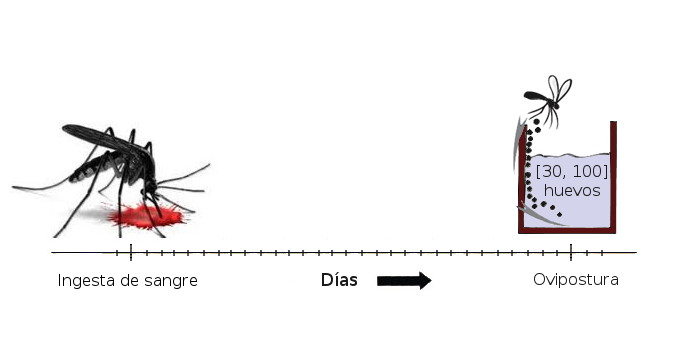
\includegraphics[width=9.5cm]{./graphics/cliclo-gonotrofico-tiempo.jpg}
  \end{center}
\end{frame}

\begin{frame}[t]{Modelos de simulación de la ecología del vector.\\\textit{Dispersión.}}
  \begin{center}
    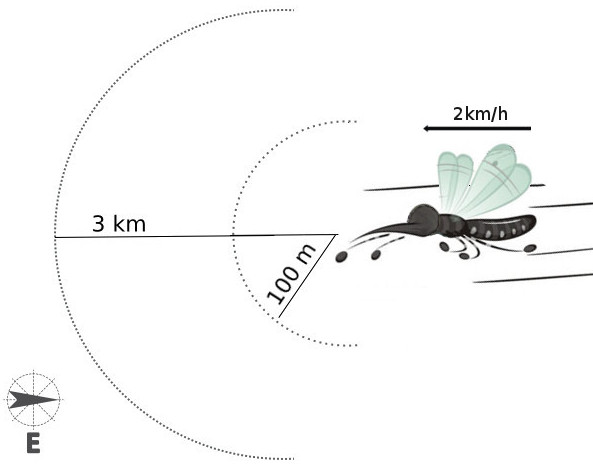
\includegraphics[width=7.5cm]{./graphics/dispersion.jpg}
  \end{center}
\end{frame}

\begin{frame}[c]{Simulación del proceso evolutivo}
  \begin{center}
    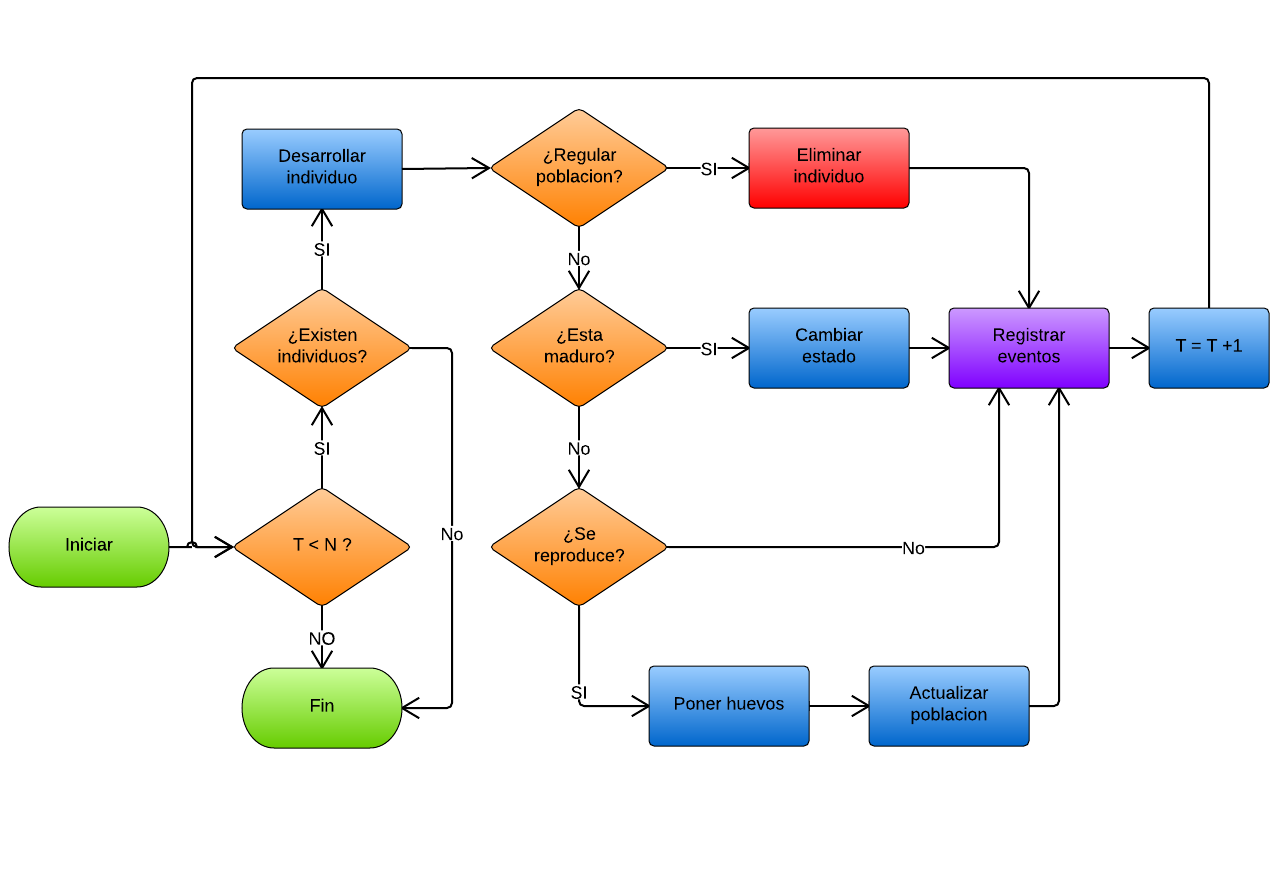
\includegraphics[height=7.5cm]{./graphics/algoritmo-propuesto.png}
  \end{center}
\end{frame}

